%%%%%%%%%%%%%%%%%%%%%%%%%%%%%%%%%%%%%%%%%%%%%%%%%%%%%%%%%%%%%%%%%%%%%%%%%%%%%%%
%% StuPro A, Produktlinien (Kobold)
%% Team Werkbold
%% Grobentwurf
%% $Id: grobentwurf.tex,v 1.1 2004/03/01 01:51:07 vanto Exp $
%%%%%%%%%%%%%%%%%%%%%%%%%%%%%%%%%%%%%%%%%%%%%%%%%%%%%%%%%%%%%%%%%%%%%%%%%%%%%%%
\documentclass[a4paper,titlepage,12pt,ngerman]{scrbook}
\usepackage{../common/header}
\usepackage{supertabular}

\RCSdef $Revision: 1.1 $
\RCSdef $Date: 2004/03/01 01:51:07 $

%\newcommand\version{Version \today \xspace}
\newcommand\version{Version 1.0\xspace}

\title {\huge \product\\[0.5cm]\large Spezifikation I \\[0.5cm] \version
  \\[1cm] \Large \company}

\begin{document}

%%%%%%%%%%%%%%%%%%%%%%%%%%%%%%%%%%%%%%%%%%%%%%%%%%%%%%%%%%%%%%%%%%%%%%%%%%%%%%%
%% Deckblatt

\begin{titlepage}
\renewcommand{\thefootnote}{\fnsymbol{footnote}}
{\Huge
\raggedright
\textbf{\bf Kobold} \\
\huge Produktlinien Management System
\rule{\textwidth}{0.75pt}
\par
}
\begin{flushleft}
\normalsize
\version
\end{flushleft}


\vfill

\includegraphics[width=15cm]{../common/logo-color.png}
\vfill
{\parindent=0cm
\Huge Grobentwurf I
}


\setcounter{footnote}{0}
\end{titlepage}

%%%%%%%%%%%%%%%%%%%%%%%%%%%%%%%%%%%%%%%%%%%%%%%%%%%%%%%%%%%%%%%%%%%%%%%%%%%%%%%
%% Versionsgeschichte

\section*{Versionsgeschichte}

\begin{itemize}

\item Version 1.0 (20.02.2004)
    
    Diese Version wurde dem Auftraggeber vorgelegt.

\end{itemize}

%%%%%%%%%%%%%%%%%%%%%%%%%%%%%%%%%%%%%%%%%%%%%%%%%%%%%%%%%%%%%%%%%%%%%%%%%%%%%%%
%% Inhaltsverzeichnis
\tableofcontents
%%%%%%%%%%%%%%%%%%%%%%%%%%%%%%%%%%%%%%%%%%%%%%%%%%%%%%%%%%%%%%%%%%%%%%%%%%%%%%%%%%% 
\chapter{Einleitung}

\section{�ber dieses Dokument}

Diese Spezifikation dient als Grundlage zur informalen
Beschreibung des Produktlinien Management Systems \product.
Aufgrund des evolution�ren Vorgehensmodells wird dieses Dokument
iterativ erweitert und verfeinert und zu Beginn jeder
Folge-Iteration der weiteren Entwicklung zugrundegelegt.\par Das
Dokument richtet sich sowohl an den Auftraggeber und dessen
technische Berater als auch an die Mitarbeiter des
Werkbold-Teams.\par Es wird vom Auftraggeber am Anfang jeder
Iteration abgenommen und ist von da an Vertragsbestandteil f�r die
weitere Entwicklung von \product.

\subsection{Spezifikation I}
Die Spezifikation I dient als Grundlage zur informalen
Beschreibung des Rahmensystems von \product, das in der ersten
Iteration entwickelt wird.\par Sie basiert auf der Abstraktion der
ermittelten Anforderungen an das Produktlinien Management System
\product (vgl. Anhang B).\par Aufgrund des abstrakten Charakters
der Spezifikation des Rahmensystems wird auf eine explizite
Spezifikation von Use-Cases verzichtet. Diese wird Gegenstand der
Spezifikationen in den Folge-Iterationen sein.

\section{Das Kobold-System}

Das wesentliche Einsatzziel des Produktlininen Management Systems
\product ist die werkzeugunterst�tzte Entwicklung und Pflege von
Software-Produktlinien und die Etablierung eines rollenbasierten
Entwicklungsprozesses.


\subsection{Grundlegende Architekturentscheindungen}
Die grundlegende Architektur von \product untergliedert sich in
zwei Teilsysteme: der Kobold Client, der als rollenbasierte
Entwicklungsumgebung f�r die Verwaltung von Produktlinien und
Produkten konzipiert ist, und dem Kobold Server-Dienst, der die
Benutzer-, Rollen- und Nachrichten-Verwaltung erm�glicht. \par Der
Eclipse-basierte Client bietet dem Benutzer eine graphische
Benutzungsoberfl�che, �ber die er seine Produktlinien und Produkte
rollenabh�ngig verwalten kann. Er kann damit seine Architekturen
als Graphen ansehen und ver�ndern, neue Rollen verteilen,
Nachrichten verschicken und Workflows ausl�sen.\par Der Server
verwaltet die Daten der einzelnen Benutzer und deren
Zugriffsrechte. Er bietet den Clients au�erdem einen zentralen
Nachrichtendienst an. Wenn von einem Client eine Nachricht an den
Serverdienst gesendet wird, pr�ft der Serverdienst die Nachricht
auf m�gliche Konsequenzen, die anderen Clients in Form von
Workflows zugeteilt werden. Dar�ber hinaus verwaltet der
Serverdienst auch die Pfade und Zugriffskonfigurationen der
Repositories, in denen die Daten der Produkte und Produktlinien
gespeichert und versioniert werden.

\chapter{Der Kobold Client}
Der Client basiert grundlegend auf der Eclipse Plattform und deren Widgettoolkit und ist
dadurch von dessen nativer Schnittstelle abh�ngig. Laut dem Eclipse Consortium werden die folgenden 
Plattformen und Betriebssysteme unterst�tzt:
\begin{itemize}
    \item Windows NT/2000/XP
    \item Linux (x86/Motif)
    \item Linux (x86/GTK 2)
    \item Solaris 8 (SPARC/Motif)
    \item QNX (x86/Photon)
    \item AIX (PPC/Motif) 
    \item HP-UX (HP9000/Motif)
    \item Mac OSX (Mac/Carbon)
\end{itemize}
Er wird als Feature-Set implementiert und mit eigenem Product Branding versehen.
Das Product Branding umfasst die �nderung der Fensternamen und der Produkticons, sowie
einer Willkommensseite die einen kurzen �berblik �ber Funktionalit�t und Zweck des Kobold Tools geben soll.

Das Feature-Set wird als Set von inernationalisierbaren Eclipse Plugins implementiert.
Die Ausgangsperspektive wird aus 4 Teilen bestehen:
\begin{itemize}
	\item Der Produktlinienarchitektur View/Editor
	\item Der Rollen View
	\item Der Worklflow/Task View
	\item Die Minimap
\end{itemize}
Diese werden in den jeweiligen Unterkapiteln n�her beschrieben.
Um das Rollenprinzip konsistent durchzusetzen ist eine zentrale Anmeldung an einem Server n�tig.
Details zu der Serverseitigen L�sung finden sie auf Seite %todo Link zur Serverseite% 
. 
\section{Authentifizierung}
Die Authentifizierung am Server erfolgt durch einen RPC. Der Benutzer kann bei der Erstbenutzung des 
Clients w�hlen ob er sich bei jedem Programmstart authentifiziern will, oder ob das Passwort
und der Benutzername gespeichert werden sollen. Prinzipiell ist ein �ndern von Daten im nichtauthentifizierten
Zustand nicht m�glich. Mit der Authentifizierung werden die Rollen die dem Benutzer zugeteilt sind,
an den Client �bergeben, der Client reagiert seinerseits mit dem Bereitstellen der relevanten Sichten/
Views f�r den Benutzer.
\section{Der Produktlinienarchitektur View/Editor}
In diesem View wird die je nach aktiver Rolle relevante Sicht auf die Architektur der Produktlinie
angezeigt. Die grafische "Notation" h�lt sich dabei an die in dem Paper ... festgelegte Struktur.
Um dies nocheinmal grafisch darzustellen hier noch einmal die 3 verschiedenen Sichten auf die
Produktlinien bzw. Produktarchitektur.
Die Ansicht bietet die M�glichkeit verschidene Zoomstufen einzustellen. Dies reultiert darin,
dass im aktuellen Ausschnitt m�glicherweise nicht die ganze Architektur zu sehen ist.
Um trotzdem den �berblick zu gew�hrleisten wird eine Minimap zur Verf�gung gestellt.

%todo Grafiken einf�gen%
\subsection{Ansicht der Rolle ProduktlinienIngenieur}

\begin{figure}[ht]
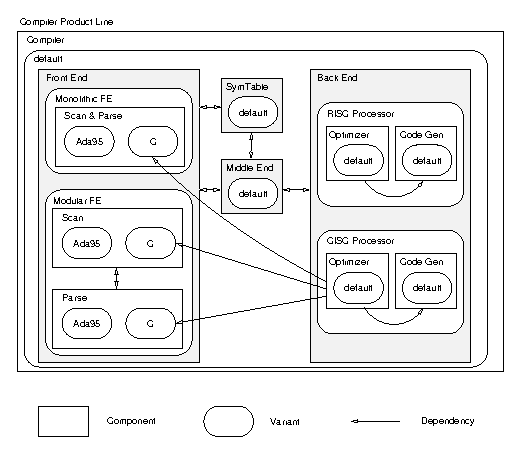
\includegraphics[width=15cm]{compiler-spl}
   \caption{Sicht des Produktlinieningenieurs}
\end{figure}
\subsection{Ansicht der Rolle eines Produktingenieurs}
\begin{figure}[ht]
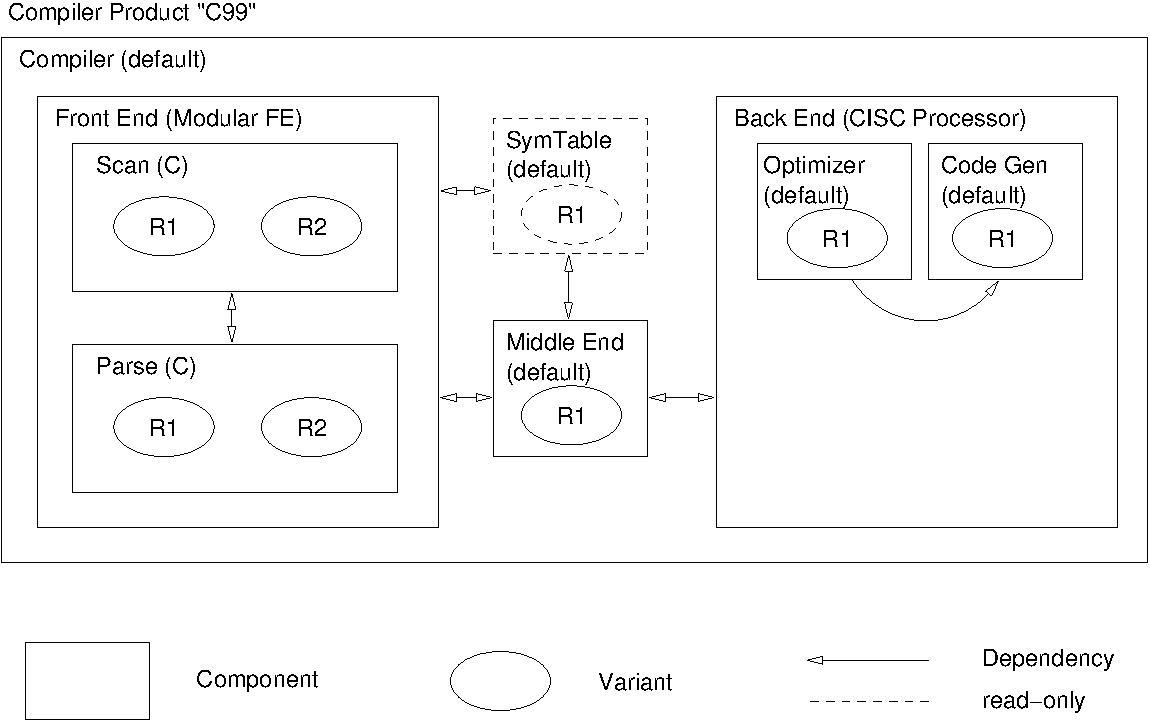
\includegraphics[width=15cm]{compiler-pe}
   \caption{Sicht des Produktingenieurs}
\end{figure}
\subsection{Ansicht der Rolle eines Programmierers}
\begin{figure}[ht]
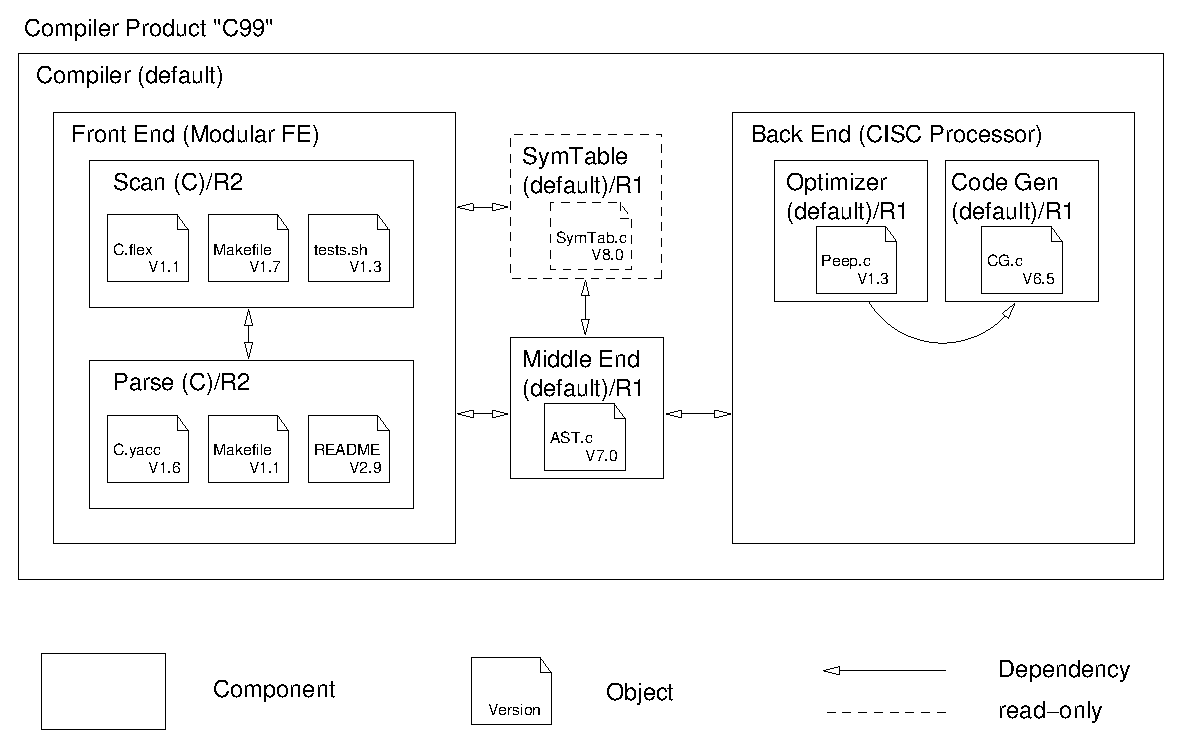
\includegraphics[width=15cm]{compiler-p}
   \caption{Sicht des Programmierers}
\end{figure}

\section{Der Rollen View}
Auf der linken Seite der Ausgangsperspektive wird ein hierarchischer Baum angezeigt, der
die momentan aktive Rolle und die mit Ihr verbundenen m�glichen Sichten darstellt.
\section{Der Worklflow/Task View}
Am unteren Rand der Ausgangsperspektive wird standardm�ssig 
\section{Die Minimap}
Am rechten unteren Rand der Ausgangsperspektive wird eine sogennante Minimap angezeigt,
in der ein �berblick �ber die ganze Architektursicht der aktuellen Rolle gegeben wird.

\chapter{Server}

Dieser Abschnitt beschreibt die Komponenten des Entwurfs des
Kobold Servers. In der Iteratrion 1 untergliedert sich der Server
in 5 Komponenten. Man beachte insbesondere auch das Kapitel 2.3
der Spezifikation1, das die Anforderungen an die jeweiligen
Komponenten spezifiziert.

\section{�berblick}
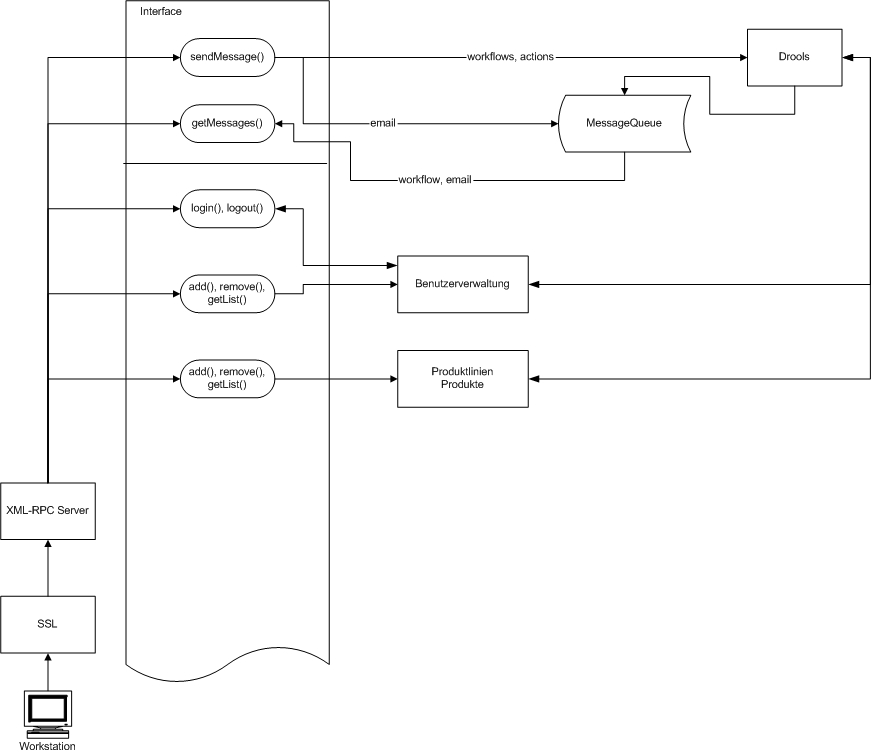
\includegraphics[width=15cm]{server.jpg}

\section{Komponente Kobold Interface}

Die Komponente Interface bildet die Schnittstelle des Kobold
Servers nach aussen und ist dessen Einsprungklasse. Sie wird von
den Kobold Clients �ber remote procedure calls angesprochen.
Anfragen werden an die daf�r zust�ndigen Komponenten des Kobold
Servers delegiert.

\section{Komponente WorkflowEngine}

Diese Komponente erh�lt Daten �ber durchgef�hrte (VCM-)Actionen
sowie Workflowobjekte, die auf die vorhandenen Regelmengen
angewendet werden. Daf�r k�nnen ben�tigte Daten von den
Komponenten Benutzerverwaltung und Produktlinienverwaltung
abgerufen werden. Als Konsequenz k�nnen Workflows oder EMails an
die MessageQueue-Komponente �bergeben werden.

\section{Komponente MessageQueue}

Aufgabe dieser Komponente ist die Verwaltung und Zustellung von
Worklows und EMails an die addressierten Clients, sobald diese
getMessages() aufrufen.

\section{Komponente Benutzerverwaltung}

Die Benutzerverwaltung ist zust�ndig f�r die Authentifizierung der
Benutzer beim Login und verwaltet deren Rollendaten. S�mtliche
Benutzerdaten k�nnen von dieser Komponente abgefragt werden.

\section{Komponente Produktlinien-/Produktverwaltung}

Diese Komponente verwaltet s�mtliche auf dem Server zu
persistierende Daten zu Produktlinien und Produkten.



%%%%%%%%%%%%%%%%%%%%%%%%%%%%%%%%%%%%%%%%%%%%%%%%%%%%%%%%%%%%%%%%%%%%%%%%%%%%%%%
%% Anhang
\appendix
%%%%%%%%%%%%%%%%%%%%%%%%%%%%%%%%%%%%%%%%%%%%%%%%%%%%%%%%%%%%%%%%%%%%%%%%%%%%%%%
%% StuPro A, Produktlinien (Kobold)
%% Team Werkbold
%% Angebot
%% $Id: begriffslexikon.tex,v 1.6 2004/02/19 14:04:10 grosseml Exp $
%%%%%%%%%%%%%%%%%%%%%%%%%%%%%%%%%%%%%%%%%%%%%%%%%%%%%%%%%%%%%%%%%%%%%%%%%%%%%%%
\newcommand{\begriff}[2]
{\item \bfseries{#1} \textnormal{#2}}

\chapter{Begriffslexikon}
\begin{itemize}

\begriff{Ansicht}{Eine rollenabh�ngige Sicht}

\begriff{Arbeitskopie}{Kopie, mit der gearbeitet wird und die tats�chlich ver�ndert wird}

\begriff{Architektur}{Struktur von Software, die aus Komponenten und
Konnektoren besteht}

\begriff{Auschecken}{VCM-Funktion zum Anfordern einer Arbeitskopie aus dem Repository}

\begriff{Assets}{Wiederverwendbare Komponenten, z.B. Source-Pakete, Klassen,
usw.}

\begriff{Core-Assets}{Architekturkomponenten, die bestimmte Funktionalit�ten 
erf�llen und oft wiederverwendet werden. Sie bilden mit den produktspezifischen 
Komponenten das Produkt}

\begriff{Core-Asset-Entwickler}{Softwareentwickler, der Core-Assets entwickelt}

\begriff{Core-Asset-Repository}{Entwicklungs-Repository (Arbeitskopie) der
Core-Assets}

\begriff{Deprecated}{Veraltet, missbilligend}

\begriff{Einchecken}{VCM-Funktion zum R�ckschreiben der Arbeitskopie-�nderungen
ins Repository}

\begriff{Entwicklungs Repository} {Siehe Arbeitskopie}

\begriff{Erstentwicklung}{Entwicklung eines neuen Produkts bzw. eines neuen 
Core-Assets}

\begriff{Evolution�res Vorgehensmodell}{Inkrementelles Vorgehensmodell in der
Softwareentwicklung, �hnlich dem Spiralmodell nach B.W. Boehm}

\begriff{Fakt}{eine Mitteilung an den Kobold-Server}

\begriff{Feature-Set}{Ein Plugin-Satz zur Erweiterung von Eclipse, so dass 
Eclipse nach der Erweiterung ein eigenes Erscheinungsbild hat}

\begriff{Iteration}{Phase im evolution�ren Vorgehensmodell}

\begriff{Kernkomponenten}{siehe Core-Assets}

\begriff{Komponenten}{Bestandteile der Produktlinien- bzw. Produktarchitektur}

\begriff{Message-Queue}{Nachrichten, die auf Anfrage an den Benutzer geleitet werden}

\begriff{Metainformation}{Zusatz-Informationen �ber Informationen}

\begriff{Module}{siehe Komponenten}

\begriff{Plugin}{Softwarekomponente, die die Funktionalit�t des Systems erweitert}

\begriff{Produktarchitektur}{Software-Architektur eines Produktes}

\begriff{Produkt-Entwickler}{P, Softwareentwickler dessen Vorgesetzter ein
Produkt-Ingenieur ist}

\begriff{Produkt-Ingenieur}{PE, ein Software-Ingenieur mit Leitungs- und 
Entscheidungskompetenz bzgl. der technischen Realisierung des Produkts. 
Der PE hat den Produktlinien-Ingenieur als Vorgesetzten.}

\begriff{Produktlinien-Ingenieur}{PLE, Software-Ingenieur mit projekt�bergreifender 
Leitungs- und Entscheidungskompetenz bzgl. der technischen Realisierung 
und Pflege der Produktlinienarchitektur.}

\begriff{Produkt-Repository}{Repository, das vom PE verwaltet wird, Entwickler
checken Arbeitskopien von Produkt�Komponenten aus}

\begriff{Produktlinien-Repository}{Repository, das vom PLE verwaltet wird, PE checken
Arbeitskopien von Core-Asset Varianten aus}

\begriff{Prototyp}{Entwicklungsversion eines Programmes}

\begriff{RPC}{Remote Procedure Call erlaubt die Ausf�hrung von Funktionen, 
die auf einem anderen Rechner implementiert sind}

\begriff{Repository}{Datei-Verwaltung zur Verwaltung von Versionen}

\begriff{Softwarearchitektur}{siehe Architektur}

\begriff{Update}{VCM-Funktion, die die Arbeitskopie mit dem Repository
synchronisiert}

\begriff{Varianten}{Modifikationen von Core-Assets}

\begriff{VCM}{Version Control Management, ein Versionsverwaltungssystem wie z.B.
das Versionsverwaltungstool CVS (Concurrent Versions System)}

\begriff{Version}{Eindeutige Bezeichnung zu einem fixen Zeitpunkt}

\begriff{View}{Subfenster von Kobold-Client}

\begriff{Wasserfall-Vorgehensmodell}{Klassisches Vorgehensmodell in der
Softwareentwicklung, das in Phasen aufgeteilt ist, die aufeinander folgen}

\begriff{Workflow}{Arbeits- bzw. Gesch�ftsprozess}

\end{itemize}

%%% Local Variables: 
%%% TeX-master: "angebot"
%%% End: 
%%% vim:tw=79:


\end{document}
%%% vim:tw=79:
